\chapter{La plante domestiquée}\label{ch:g12:domesticated-plants}

À côté d'un épi de maïs moderne --- six cents grains en rangées bien
ordonnées, enveloppés de spathes, tenus sur une rafle qui ne les
lâchera pas --- on avait posé l'épi de téosinte, la graminée sauvage
dont il vient~: une douzaine de grains sur une seule rangée, chacun
enfermé dans une coque pierreuse, tombant un à un à maturité. Neuf
mille ans de choix, faits par des cultivateurs qui gardaient les
graines des plantes qu'ils préféraient, ont transformé l'un en
l'autre. Le résultat ne peut pas survivre une saison sans nous~: un
épi de maïs laissé dans un champ pourrit sur place. Ce chapitre traite
de ce qui arrive à une plante quand les humains deviennent son milieu
sélectif --- et des manières plus récentes de modifier à dessein les
\omterm{def:g10:universal-dna:gene}{gènes} d'une plante.

\section{La sélection par les humains}

\begin{definition}[Domestication, sélection artificielle]\label{def:g12:domesticated-plants:domestication}
La \emph{domestication}\index{domestication} est la transformation
d'une \omterm{def:g10:biodiversity-scales:species}{espèce} sauvage en une \omterm{def:g10:biodiversity-scales:species}{espèce} qui dépend des humains et les sert,
par \emph{sélection artificielle}\index{sélection artificielle}~: à
chaque génération, les humains conservent et sèment les graines des
individus qui portent les caractères qu'ils veulent, de sorte que les
\omterm{def:g10:universal-dna:gene}{allèles} responsables de ces caractères augmentent en fréquence. C'est
la sélection du \cref{ch:g12:selection-drift-speciation} avec un œil
humain à la place du milieu, et elle obéit à la même
arithmétique --- en plus rapide, puisque le choix est délibéré et
sévère.
\end{definition}

\begin{proposition}[Ce que sélectionne la domestication]\label{prop:g12:domesticated-plants:traits}
Les plantes cultivées partagent un ensemble de caractères qu'aucune
plante sauvage ne conserverait, le \emph{syndrome de
\omterm{def:g12:domesticated-plants:domestication}{domestication}}~: des graines qui restent sur la plante au lieu de se
disperser (un épi non égrenant)~; des graines et des fruits plus
gros~; des graines qui germent aussitôt au lieu d'attendre des années
dans le sol~; la perte des toxines et des défenses amères~; une plante
compacte, peu ramifiée, portant un gros épi plutôt que de nombreux
petits~; et une maturation simultanée. Chacun est utile au moissonneur
et nuisible à une plante livrée à elle-même --- une plante cultivée
est une plante sélectionnée pour notre commodité et contre son
indépendance.
\end{proposition}
\begin{proof}[Preuves]
Le blé sauvage laisse tomber ses grains d'un rachis cassant~; les
premiers blés cultivés, trouvés dans les plus anciens sites agricoles,
ont un rachis solide qui retient le grain --- la faucille du
moissonneur a sélectionné, sans le vouloir, les mutants dont le grain
restait sur la plante pour être récolté et semé. La téosinte et le
maïs ne diffèrent que par cinq \omterm{def:g10:universal-dna:gene}{gènes} majeurs environ~: l'un transforme
une plante très ramifiée en une tige unique, un autre libère le grain
de sa coque pierreuse, d'autres multiplient les rangées. Le croisement
des deux donne une descendance féconde, et les formes intermédiaires
existent~: la même \omterm{def:g10:biodiversity-scales:species}{espèce}, remodelée.
\end{proof}

\begin{omfigure}
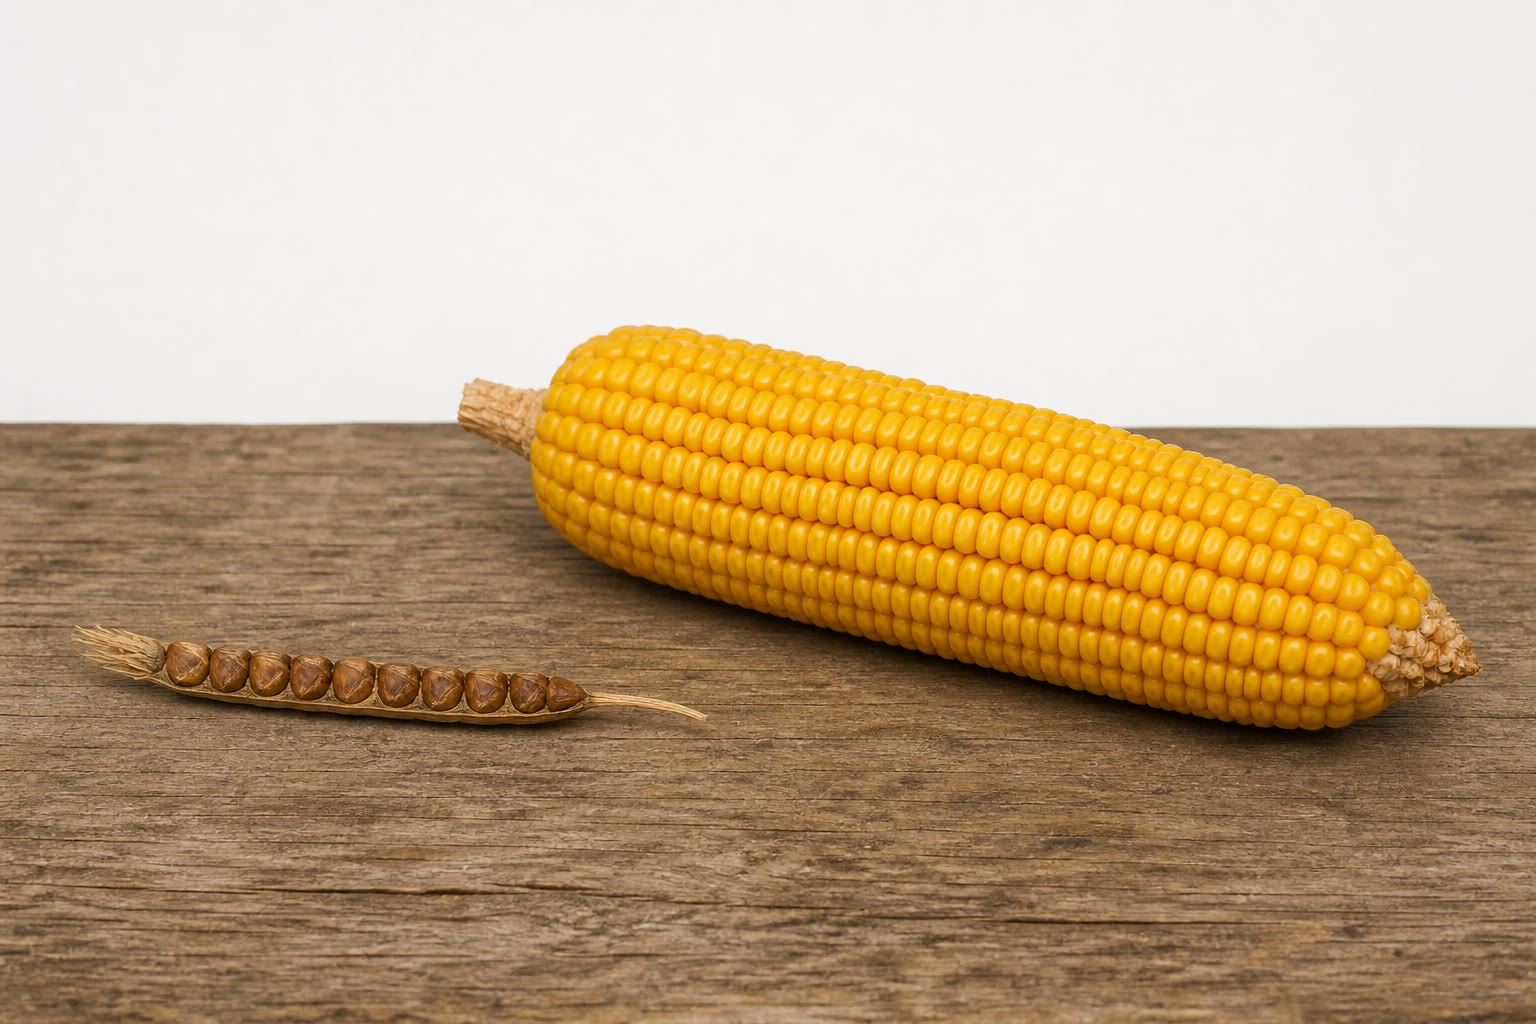
\includegraphics[width=0.62\linewidth]{images/book2/ai/g12-domestic-teosinte-maize.jpg}

{\small La téosinte et le maïs. Une douzaine de grains en coque sur
une seule rangée le long d'un axe cassant, face à des centaines de
grains nus solidement tenus sur une rafle~: neuf mille ans de choix,
et une poignée de \omterm{def:g10:universal-dna:gene}{gènes}.}
\end{omfigure}

\begin{omfigure}
\begin{tikzpicture}[font=\small, >=Stealth,
  b/.style={draw, rounded corners, align=center, text width=2.2cm, minimum height=0.9cm}]
  \node[b, fill=omMeth!15, text width=2.8cm] (wild) at (0,0) {chou sauvage\\ (une seule espèce)};
  \node[b, fill=omDef!12] (kale) at (5,3.0) {chou frisé~:\\ feuilles};
  \node[b, fill=omDef!12] (cab) at (5,1.8) {chou pommé~:\\ bourgeon terminal};
  \node[b, fill=omDef!12, text width=2.7cm] (spr) at (5,0.6) {chou de Bruxelles~:\\ bourgeons latéraux};
  \node[b, fill=omDef!12] (kohl) at (5,-0.6) {chou-rave~:\\ tige};
  \node[b, fill=omDef!12] (broc) at (5,-1.8) {brocoli~:\\ boutons floraux};
  \node[b, fill=omDef!12] (cauli) at (5,-3.0) {chou-fleur~:\\ pédoncules floraux};
  \foreach \t in {kale,cab,spr,kohl,broc,cauli} \draw[->] (wild.east) -- (\t.west);
  \node[anchor=west, align=left, text width=4.6cm] at (7.2,0) {Six plantes cultivées, une seule espèce~: dans chaque lignée, les cultivateurs ont sélectionné l'exagération d'un organe différent. Toutes les six se croisent encore entre elles.};
\end{tikzpicture}

{\small La \omterm{def:g12:domesticated-plants:domestication}{sélection artificielle} à partir d'une seule \omterm{def:g10:biodiversity-scales:species}{espèce} sauvage.
Sélectionner les feuilles, les bourgeons, la tige ou les fleurs dans
des lignées différentes a produit des plantes qui ressemblent à des
\omterm{def:g10:biodiversity-scales:species}{espèces} différentes sans en être.}
\end{omfigure}

\begin{example}[Ce qu'une plante cultivée a perdu]\label{ex:g12:domesticated-plants:lost}
Le maïs ne peut pas disperser ses graines~; le blé cultivé ne peut pas
laisser tomber son grain~; la banane et le raisin sans pépins ne font
aucune graine et se multiplient par bouturage, chaque plante étant un
clone. La survie d'une plante cultivée est déléguée au cultivateur, et
sa \emph{\omterm{def:g10:biodiversity-scales:biodiversity}{diversité génétique}} s'est réduite à chaque étape de la
sélection~: une variété moderne est presque uniforme, et une région
entière peut n'en cultiver qu'une seule. Les parents sauvages, encore
divers, sont le lieu où se conservent les \omterm{def:g10:universal-dna:gene}{allèles} dont une plante
cultivée pourra avoir besoin demain --- pour une nouvelle maladie, un
climat plus sec (\cref{ch:g10:biodiversity-scales}).
\end{example}

\section{Améliorer par croisement}

\begin{proposition}[Variétés et hybrides]\label{prop:g12:domesticated-plants:hybrids}
Les sélectionneurs créent de nouvelles variétés en croisant des
plantes porteuses d'\omterm{def:g10:universal-dna:gene}{allèles} utiles différents et en retenant, parmi
les descendants, les combinaisons qu'ils veulent, sur plusieurs
générations. Un cas particulier domine le maïs et beaucoup de
légumes~: l'\emph{hybride F1}\index{hybride F1}. Deux lignées
pures --- rendues uniformes et homozygotes par des générations
d'autopollinisation --- sont croisées~; leurs descendants sont tous
génétiquement identiques, hétérozygotes pour chaque \omterm{def:g10:universal-dna:gene}{gène} où les
lignées diffèrent, et nettement plus vigoureux et plus productifs que
l'un et l'autre parent. Ressemée, la graine de l'hybride disjoint en
un mélange de plantes moins vigoureuses~: le cultivateur achète chaque
année de nouvelles semences hybrides.
\end{proposition}
\admitted

\begin{omfigure}
\begin{tikzpicture}[font=\small, >=Stealth,
  b/.style={draw, rounded corners, align=center, text width=2.6cm, minimum height=1.0cm}]
  \node[b, fill=omDef!12] (a) at (0,1.2) {lignée pure A\\ $AA\,bb$, uniforme};
  \node[b, fill=omDef!12] (bb) at (0,-1.2) {lignée pure B\\ $aa\,BB$, uniforme};
  \node[b, fill=omMeth!20, text width=3.0cm] (f1) at (4.6,0) {hybride F1\\ $Aa\,Bb$, tous identiques,\\ vigoureux};
  \node[b, fill=omProp!15, text width=3.4cm] (f2) at (9.6,0) {F2 issue de la graine de l'hybride~:\\ $AA$, $Aa$, $aa$ \dots mêlés,\\ rendement en baisse de 15--20\%};
  \draw[->] (a) -- (f1); \draw[->] (bb) -- (f1);
  \draw[->] (f1) -- node[above] {ressemée} (f2);
\end{tikzpicture}

{\small L'\omterm{prop:g12:domesticated-plants:hybrids}{hybride F1}. Deux lignées homozygotes donnent une descendance
hétérozygote uniforme et très vigoureuse~; la génération suivante
disjoint et perd cette vigueur, si bien que la semence doit être
rachetée chaque année --- le fondement de l'industrie semencière.}
\end{omfigure}

\begin{omfigure}
\begin{tikzpicture}
\begin{axis}[
  width=0.86\linewidth, height=5.6cm,
  axis x line=bottom, axis y line=left,
  xmin=1900, xmax=2025, ymin=0, ymax=9,
  xlabel={année}, ylabel={rendement du blé (t/ha)},
  xlabel style={font=\small, at={(axis description cs:0.5,-0.12)}, anchor=north},
  ylabel style={font=\small},
  tick label style={font=\small}, xtick={1900,1925,1950,1975,2000,2025}, ytick={0,2,4,6,8},
  clip=false,
]
\addplot[thick, omMeth, mark=*, mark size=1.5pt] coordinates
  {(1900,1.3) (1920,1.4) (1940,1.6) (1950,1.9) (1960,2.6) (1970,3.6) (1980,5.0) (1990,6.5) (2000,7.2) (2010,7.3) (2020,7.5)};
\draw[dashed, gray] (axis cs:1955,0) -- (axis cs:1955,8.5);
\node[font=\scriptsize, anchor=south, align=center] at (axis cs:1955,8.5) {variétés à paille courte,\\ engrais, pesticides};
\end{axis}
\end{tikzpicture}

{\small Rendement moyen du blé dans un pays d'Europe occidentale au
cours d'un siècle (valeurs arrondies). Stable pendant cinquante ans,
il a quadruplé en quarante ans grâce à de nouvelles variétés créées
pour porter de lourds épis sur des tiges courtes, avec l'engrais et la
lutte contre les ravageurs. Le plateau observé depuis 2000 est l'objet
des travaux de sélection actuels.}
\end{omfigure}

\begin{example}[Pourquoi l'hybride est vigoureux, et pourquoi cela ne dure pas]\label{ex:g12:domesticated-plants:vigour}
Chaque lignée pure, homozygote partout, porte en double dose quelques
\omterm{def:g10:universal-dna:gene}{allèles} \omterm{def:g11:genes-and-disease:genetic}{récessifs} défavorables~; croiser deux lignées masque les
\omterm{def:g10:universal-dna:gene}{allèles} défavorables de chacune derrière les \omterm{def:g10:universal-dna:gene}{allèles} fonctionnels de
l'autre, pour chaque \omterm{def:g10:universal-dna:gene}{gène} où elles diffèrent. La F1 est donc
hétérozygote et vigoureuse. À la génération suivante, la \omterm{def:g12:meiosis-genetic-shuffling:meiosis}{méiose} et la
fécondation redistribuent les \omterm{def:g10:universal-dna:gene}{allèles}
(\cref{ch:g12:meiosis-genetic-shuffling})~: un quart des plantes est
homozygote pour l'\omterm{def:g10:universal-dna:gene}{allèle} défavorable à chaque \omterm{def:g10:universal-dna:gene}{gène}, et le champ
devient une mosaïque.
\end{example}

\section{Modifier les gènes directement}

\begin{proposition}[Plantes transgéniques et plantes éditées]\label{prop:g12:domesticated-plants:transgenic}
Depuis les années 1980, un \omterm{def:g10:universal-dna:gene}{gène} peut être introduit dans une plante
sans croisement~: c'est la \emph{transgenèse}\index{transgenèse}
(\cref{ch:g10:universal-dna}). Une bactérie du sol qui injecte
naturellement un fragment de son \omterm{def:g10:universal-dna:information}{ADN} dans les \omterm{def:g10:cells-common-unit:cell}{cellules} végétales sert
de véhicule~: le \omterm{def:g10:universal-dna:gene}{gène} voulu est inséré dans ce fragment, des \omterm{def:g10:cells-common-unit:cell}{cellules}
végétales sont infectées, et des plantes entières sont régénérées à
partir des \omterm{def:g10:cells-common-unit:cell}{cellules} qui ont pris le \omterm{def:g10:universal-dna:gene}{gène}. Le \omterm{def:g10:universal-dna:gene}{gène} peut provenir de
n'importe quelle \omterm{def:g10:biodiversity-scales:species}{espèce}. Plus récemment, les \omterm{def:g10:universal-dna:gene}{gènes} propres d'une
plante peuvent être modifiés en un point choisi --- c'est
l'\emph{édition du génome} --- sans ajout d'\omterm{def:g10:universal-dna:information}{ADN} étranger. Caractères
obtenus jusqu'ici~: la résistance à un insecte (un \omterm{def:g10:universal-dna:gene}{gène} de toxine
bactérienne), la tolérance à un herbicide, la résistance à un virus,
un précurseur de vitamine dans le riz, des huiles de composition
modifiée.
\end{proposition}
\admitted

\begin{omfigure}
\begin{tikzpicture}[font=\small, >=Stealth,
  b/.style={draw, rounded corners, align=center, text width=2.4cm, minimum height=1.0cm}]
  \node[b, fill=omThm!12] (gene) at (0,0) {gène d'intérêt\\ (espèce quelconque)};
  \node[b, fill=omProp!15] (bact) at (3.3,0) {inséré dans l'ADN\\ qu'une bactérie du sol\\ transfère aux plantes};
  \node[b, fill=omDef!12] (cells) at (6.6,0) {cellules végétales infectées~;\\ certaines captent\\ le gène};
  \node[b, fill=omMeth!15] (plant) at (9.9,0) {plantes entières régénérées\\ à partir de ces cellules~:\\ transgéniques};
  \draw[->] (gene) -- (bact); \draw[->] (bact) -- (cells); \draw[->] (cells) -- (plant);
\end{tikzpicture}

{\small La fabrication d'une plante transgénique. Une bactérie qui
insère naturellement de l'\omterm{def:g10:universal-dna:information}{ADN} dans les \omterm{def:g10:cells-common-unit:cell}{cellules} végétales y fait
entrer le \omterm{def:g10:universal-dna:gene}{gène} choisi~; des plantes sont régénérées à partir des
\omterm{def:g10:cells-common-unit:cell}{cellules} qui l'ont reçu, et le transmettent par leurs graines.}
\end{omfigure}

\begin{example}[Un gène de toxine dans le maïs]\label{ex:g12:domesticated-plants:bt}
Une bactérie du sol fabrique une \omterm{def:g11:gene-expression:protein}{protéine} toxique pour les chenilles
et inoffensive pour les mammifères~; son \omterm{def:g10:universal-dna:gene}{gène}, inséré dans le maïs,
fait produire la toxine par chaque \omterm{def:g10:cells-common-unit:cell}{cellule} de la plante, et les
chenilles de pyrale qui creusent les tiges meurent à la première
bouchée. Les pulvérisations d'insecticide diminuent~; les rendements
montent là où la pyrale sévissait. En une décennie, des pyrales
résistantes à la toxine sont apparues là où la culture était menée
sans interruption --- la sélection du
\cref{ch:g11:antibiotic-resistance} dans un champ --- et les
cultivateurs sont désormais tenus de semer des refuges de maïs
ordinaire à côté du maïs transgénique, afin que des pyrales sensibles
survivent et diluent les résistantes.
\end{example}

\section{Des choix}

\begin{proposition}[Ce qui est en jeu]\label{prop:g12:domesticated-plants:stakes}
Chaque technique de ce chapitre pose les mêmes questions sous une
forme nouvelle~: le rétrécissement de la diversité (une seule variété
sur toute une région, un seul \omterm{def:g10:universal-dna:gene}{gène} dans chaque plante), la dépendance
des cultivateurs à l'égard de semences qu'ils ne peuvent pas
conserver, la sélection de ravageurs et d'adventices résistants aux
défenses de la culture, le passage des \omterm{def:g10:universal-dna:gene}{gènes} d'une plante cultivée à
ses parents sauvages par le pollen, et la sûreté comme la propriété de
ce que l'on mange. La biologie seule n'en tranche aucune~; elle dit ce
que chaque technique fait et ne fait pas, et ce qu'elle sélectionne.
\end{proposition}
\admitted

\begin{method}[Lire l'histoire d'une plante cultivée]\label{met:g12:domesticated-plants:read}
\begin{enumerate}
  \item Identifier l'ancêtre sauvage et ce que la plante cultivée a
        perdu par rapport à lui (dissémination, dormance, défenses,
        diversité).
  \item Identifier comment le changement a été obtenu~: sélection
        involontaire par la moisson, sélection délibérée, croisement
        et sélection, hybridation, \omterm{prop:g10:universal-dna:universal}{transgenèse}, édition.
  \item Compter les \omterm{def:g10:universal-dna:gene}{gènes} en jeu lorsqu'on les connaît~: quelques
        \omterm{def:g10:universal-dna:gene}{gènes} majeurs pour le syndrome de \omterm{def:g12:domesticated-plants:domestication}{domestication}, un grand
        nombre de \omterm{def:g10:universal-dna:gene}{gènes} à faible effet pour le rendement, un seul pour
        un caractère transgénique.
  \item Se demander de quoi la plante cultivée dépend désormais (le
        cultivateur, la semence achetée, un herbicide, des refuges) et
        ce qui dépend d'elle.
\end{enumerate}
\end{method}

\begin{remark}[La plus ancienne expérience d'évolution]\label{rem:g12:domesticated-plants:oldest}
Darwin a ouvert son livre sur l'origine des \omterm{def:g10:biodiversity-scales:species}{espèces} par un chapitre
sur les pigeons et les choux, parce que les éleveurs et les
sélectionneurs avaient déjà montré ce que la sélection pouvait faire
en quelques siècles~; il ne lui restait qu'à retirer le sélectionneur
et à allonger la durée. Chaque plante cultivée est une démonstration
des trois derniers chapitres --- variation, sélection, et un
changement de fréquences qui modifie une \omterm{def:g10:biodiversity-scales:species}{espèce} --- menée à la vitesse
humaine, avec le relevé des résultats dans chaque champ et sur chaque
marché.
\end{remark}

\section{Exercices}

\begin{exercise}[$\star$]\label{exo:g12:domesticated-plants:1}
Définir la \omterm{def:g12:domesticated-plants:domestication}{domestication} et la \omterm{def:g12:domesticated-plants:domestication}{sélection artificielle}.
\end{exercise}

\begin{exercise}[$\star$]\label{exo:g12:domesticated-plants:2}
Énumérer quatre caractères du syndrome de \omterm{def:g12:domesticated-plants:domestication}{domestication} et dire
pourquoi chacun est un handicap pour une plante sauvage.
\end{exercise}

\begin{exercise}[$\star$]\label{exo:g12:domesticated-plants:3}
Qu'est-ce qu'un \omterm{prop:g12:domesticated-plants:hybrids}{hybride F1}, et pourquoi les cultivateurs en
achètent-ils la semence chaque année~?
\end{exercise}

\begin{exercise}[$\star$]\label{exo:g12:domesticated-plants:4}
Comment introduit-on un \omterm{def:g10:universal-dna:gene}{gène} dans une plante sans croisement~?
\end{exercise}

\begin{exercise}[$\star$]\label{exo:g12:domesticated-plants:5}
D'après la figure des rendements, par quel facteur le rendement du blé
a-t-il augmenté entre 1950 et 2000~?
\end{exercise}

\begin{exercise}[$\star\star$]\label{exo:g12:domesticated-plants:6}
Expliquer comment la moisson à la faucille, sans aucune intention de
sélectionner, a sélectionné un blé au rachis solide.
\end{exercise}

\begin{exercise}[$\star\star$]\label{exo:g12:domesticated-plants:7}
Le chou frisé, le chou pommé et le brocoli se croisent librement.
Forment-ils une seule \omterm{def:g10:biodiversity-scales:species}{espèce} ou trois~? Qu'est-ce qui les a rendus si
différents d'aspect~?
\end{exercise}

\begin{exercise}[$\star\star$]\label{exo:g12:domesticated-plants:8}
Deux lignées pures sont croisées. Pour un \omterm{def:g10:universal-dna:gene}{gène} où la lignée A est
$AA$ et la lignée B $aa$, donner le \omterm{def:g11:enzymes-and-phenotype:phenotype}{génotype} de la F1, puis les
\omterm{def:g11:enzymes-and-phenotype:phenotype}{génotypes} et les proportions de la F2. Pourquoi la F1 est-elle
uniforme et la F2 non~?
\end{exercise}

\begin{exercise}[$\star\star$]\label{exo:g12:domesticated-plants:9}
Pourquoi des pyrales résistantes sont-elles apparues dans les champs
de maïs producteur de toxine, et comment un refuge de maïs ordinaire
les ralentit-il~?
\end{exercise}

\begin{exercise}[$\star\star$]\label{exo:g12:domesticated-plants:10}
La téosinte et le maïs diffèrent par environ cinq \omterm{def:g10:universal-dna:gene}{gènes} majeurs.
Expliquer comment si peu de \omterm{def:g10:universal-dna:gene}{gènes} peuvent changer la plante à ce
point, à l'aide du \cref{ch:g12:diversification-of-life}.
\end{exercise}

\begin{exercise}[$\star\star$]\label{exo:g12:domesticated-plants:11}
Pourquoi les parents sauvages des plantes cultivées sont-ils conservés
dans des banques de graines, alors qu'ils ne produisent presque rien~?
\end{exercise}

\begin{exercise}[$\star\star\star$]\label{exo:g12:domesticated-plants:12}
Un colza tolérant à un herbicide est cultivé à côté d'une moutarde
sauvage avec laquelle il peut se croiser. Prévoir ce qui peut se
produire au fil des ans, et nommer les processus des chapitres
précédents qui y interviennent.
\end{exercise}

\begin{exercise}[$\star\star\star$]\label{exo:g12:domesticated-plants:13}
La courbe des rendements est plate depuis 2000. Proposer deux raisons
biologiques et une raison non biologique, et dire ce qu'un
sélectionneur pourrait tenter.
\end{exercise}

\begin{exercise}[$\star\star\star$]\label{exo:g12:domesticated-plants:14}
Comparer sur trois points une variété obtenue par croisement et
sélection et une variété obtenue par \omterm{prop:g10:universal-dna:universal}{transgenèse}~: l'origine du nouvel
\omterm{def:g10:universal-dna:gene}{allèle}, le nombre de \omterm{def:g10:universal-dna:gene}{gènes} modifiés, et le temps nécessaire.
\end{exercise}

\begin{exercise}[$\star\star\star$]\label{exo:g12:domesticated-plants:15}
«~La \omterm{def:g12:domesticated-plants:domestication}{domestication} est le contraire de la \omterm{def:g12:selection-drift-speciation:selection}{sélection naturelle}.~»
Discuter en un paragraphe, avec l'arithmétique des \omterm{def:g12:selection-drift-speciation:population}{fréquences
alléliques}, l'agent de la sélection, et le sort de la plante
sélectionnée.
\end{exercise}

\section{Problème~: neuf mille ans, cinq gènes}

\begin{problem}[{Problème du week-end --- le maïs tiré de la
téosinte~: les épis comparés, la sélection mise en comptes, le
rendement d'un hybride suivi jusqu'en F2, et un gène de toxine géré
contre la résistance}]
\label{pb:g12:domesticated-plants:1}
Un épi de téosinte porte 12 grains de \qty{0.08}{g}, enfermés dans une
coque dure, sur un axe cassant~; un épi de maïs porte 600 grains de
\qty{0.3}{g}, nus, sur une rafle rigide. Le maïs a été domestiqué il y
a environ 9000 ans~; une génération dure un an.

\medskip
\noindent\textbf{Partie I --- Les épis.}
\begin{enumerate}
  \item Calculer la masse de grain par épi chez la téosinte et chez le
        maïs, et le facteur qui les sépare.
  \item Énumérer les caractères de l'épi de maïs qui relèvent du
        syndrome de \omterm{def:g12:domesticated-plants:domestication}{domestication}, et dire pour chacun pourquoi il
        serait un handicap pour une plante sauvage.
  \item Le grain en coque est commandé par un seul \omterm{def:g10:universal-dna:gene}{gène}, l'\omterm{def:g10:universal-dna:gene}{allèle}
        «~grain nu~» étant \omterm{def:g11:genes-and-disease:genetic}{récessif}. Expliquer pourquoi les premiers
        cultivateurs n'ont pu trouver de plantes à grain nu que comme
        individus rares dans leurs champs.
  \item Supposons que l'\omterm{def:g10:universal-dna:gene}{allèle} «~grain nu~» ait eu la fréquence 0.01
        dans la \omterm{def:g12:selection-drift-speciation:population}{population} sauvage. Quelle fraction des plantes
        montrait des grains nus~?
  \item Une cultivatrice ne sème que les graines de plantes à grain
        nu. Quelle est la fréquence de l'\omterm{def:g10:universal-dna:gene}{allèle} «~grain nu~» dans sa
        récolte suivante~?
\end{enumerate}

\medskip
\noindent\textbf{Partie II --- Neuf mille générations.}
\begin{enumerate}[resume]
  \item Le nombre de grains par épi est passé de 12 à 600 en 9000
        générations. Calculer le facteur d'augmentation moyen par
        génération. Pourquoi un changement si faible par génération
        suffit-il~?
  \item Le nombre de rangées de grains est commandé par de nombreux
        \omterm{def:g10:universal-dna:gene}{gènes} à faible effet. Expliquer pourquoi un tel caractère
        répond à la sélection de façon graduelle et pendant longtemps,
        alors que le caractère «~grain en coque~» a changé d'un seul
        coup.
  \item Le maïs se croise encore avec la téosinte et donne une
        descendance féconde. Forment-ils une seule \omterm{def:g10:biodiversity-scales:species}{espèce}~? Qu'a
        changé et que n'a pas changé la \omterm{def:g12:domesticated-plants:domestication}{domestication}~?
  \item Une variété moderne est génétiquement uniforme. Énoncer le
        risque qui en découle, et la ressource qui y répond.
  \item Le maïs ne peut pas disperser ses graines. Qu'implique ce fait
        sur la relation entre la plante et le cultivateur, en termes
        de sélection~?
\end{enumerate}

\medskip
\noindent\textbf{Partie III --- L'hybride.}
La lignée pure A rend \qty{5}{t/ha}, la lignée B \qty{5.5}{t/ha}, leur
\omterm{prop:g12:domesticated-plants:hybrids}{hybride F1} \qty{10}{t/ha}~; la F2 cultivée à partir de la graine de
l'hybride rend \qty{8.2}{t/ha}. La semence hybride coûte l'équivalent
de \qty{0.4}{t/ha} de maïs.
\begin{enumerate}[resume]
  \item De quel pourcentage la F1 dépasse-t-elle le meilleur parent~?
        De quel pourcentage la F2 est-elle inférieure à la F1~?
  \item Expliquer la vigueur de la F1 et la perte de la F2 à l'aide
        des \omterm{def:g11:enzymes-and-phenotype:phenotype}{génotypes} de l'\cref{ex:g12:domesticated-plants:vigour}.
  \item Un cultivateur hésite entre acheter de la semence hybride
        chaque année et conserver la graine de la F1. Comparer les
        récoltes nettes, et dire pourquoi le commerce des semenciers
        existe.
  \item Pourquoi ne peut-on pas simplement vendre les lignées pures
        aux cultivateurs pour qu'ils fassent l'hybride eux-mêmes~?
  \item Qu'a fait le système des hybrides à la \omterm{def:g10:biodiversity-scales:biodiversity}{diversité génétique} des
        champs, et à l'indépendance du cultivateur~?
\end{enumerate}

\medskip
\noindent\textbf{Partie IV --- Le \omterm{def:g10:universal-dna:gene}{gène} de toxine.}
Une \omterm{def:g12:selection-drift-speciation:population}{population} de pyrales possède un \omterm{def:g10:universal-dna:gene}{allèle} de résistance à la
fréquence 0.001, \omterm{def:g11:genes-and-disease:genetic}{récessif}~; seules les pyrales $rr$ survivent sur le
maïs à toxine.
\begin{enumerate}[resume]
  \item Quelle fraction des pyrales survit sur un champ de maïs à
        toxine la première année~? Calculer la fréquence de $r$ parmi
        les survivantes.
  \item Expliquer pourquoi, sans refuges, la résistance se répand en
        quelques années, en prenant le cas des \omterm{def:g11:antibiotic-resistance:antibiotic}{antibiotiques} pour
        modèle.
  \item Un refuge de maïs ordinaire maintient en vie une \omterm{def:g12:selection-drift-speciation:population}{population}
        nombreuse de pyrales sensibles à côté du champ à toxine.
        Expliquer comment cela maintient rare l'\omterm{def:g10:universal-dna:gene}{allèle} de résistance,
        à l'aide du \omterm{def:g11:enzymes-and-phenotype:phenotype}{génotype} des descendants d'une survivante
        résistante et d'une pyrale du refuge.
  \item Comparer le refuge avec la «~cure complète~» d'\omterm{def:g11:antibiotic-resistance:antibiotic}{antibiotiques}~:
        qu'y a-t-il de commun, qu'y a-t-il de différent~?
  \item Énoncer le résultat~: le facteur par lequel la \omterm{def:g12:domesticated-plants:domestication}{domestication} a
        multiplié le grain d'un épi, le nombre de \omterm{def:g10:universal-dna:gene}{gènes} majeurs qu'il
        y a fallu, et l'unique dépendance qu'elle a créée.
\end{enumerate}
\end{problem}
